\section{Задание №11}

Построить двумерное пуассоновское поле, отвечающее сложному пуассоновскому процессу:
\begin{enumerate}
        \item Первая интерпретация: система массового обслуживания. При этом первая координата поля --- время поступления заявки в СМО (равномерное распределение), вторая --- время её обслуживания (распределение $\chi^2$ с 10-ю степенями свободы).
        \item Вторая интерпретация: система массового обслуживания с циклической интенсивностью $\lambda(t) = \lambda_0 (1 + \cos(t))$ и единичными скачками. Свести данную задачу моделирования неоднородного пуассоновского процесса при помощи метода Льюиса и Шедлера к моделированию двумерного пуассоновского поля, где первая координата имеет равномерное распределение, а вторая --- распределение Бернулли.
        \item Третья интерпретация: работа страховой компании. Первая координата~--- момент наступления страхового случая (равномерное распределение), вторая координата~--- величина ущерба (распределение Парето). Поступление капитала по времени линейно со скоростью $c > 0$, начальный капитал $W > 0$.
        \item Для каждой системы рассмотреть всевозможные случаи поведения системы в зависимости от значения параметров.
\end{enumerate}


\subsection{Система массового обслуживания}

Пусть $\lambda$ --- интенсивность пуассоновского поля. Время поступления новых заявок генерируются таким образом, что
$$
        \Delta t_i = t_i - t_{i-1}
        \sim
        \mathrm{Exp}(\lambda).
$$

\begin{definition}
        \textit{Распределением $\chi^2$ с $k$ степенями свободы} называется распределение суммы квадратов $k$ независимых стандартных случайных величин.
\end{definition}

Время обслуживания $i$-ой заявки обозначим за $s_i$. Эти времена независимы и генерируются как случайные величины с распределением $\chi^2(10)$. Все заявки обрабатываются последовательно. Таким образом, мы можем найти время окончания обработки $i$-ой заявки $Q_i$ так:
$$
        \begin{cases}
Q_i = t_i + s_i, 
        &
\mbox{если $(i-1)$-ая заявка обработана,}
        \\
Q_i = Q_{i-1} + s_i,
        &
\mbox{иначе.}
        \end{cases}
$$
Или, обобщая, можно написать так:
$$
        Q_i
        =
        t_i
        +
        \max\{0,\,Q_{i-1} - t_i\}
        +
        s_i.
$$

Для каждой заявки, мы будем считать количество заявок, ожидающих обработки, на момент прихода данной заявки. То есть количество $n_i$ таких заявок $j$, что
$$
        j < i
        \quad
        \mbox{и}
        \quad
        Q_j > t_i.
$$

Поскольку среднее время обработки одной заявки равен $10$, а средний интервал между поступлениями заявок равен $\E\,\Delta_i = \nicefrac{1}{\lambda}$, то ожидаем отсутствия очереди при $\lambda < 0,\!1$ и неограниченный рост очереди при $\lambda > 0,\!1$.

\clearpage
\begin{figure}[t]
        \noindent
        \centering
        {
        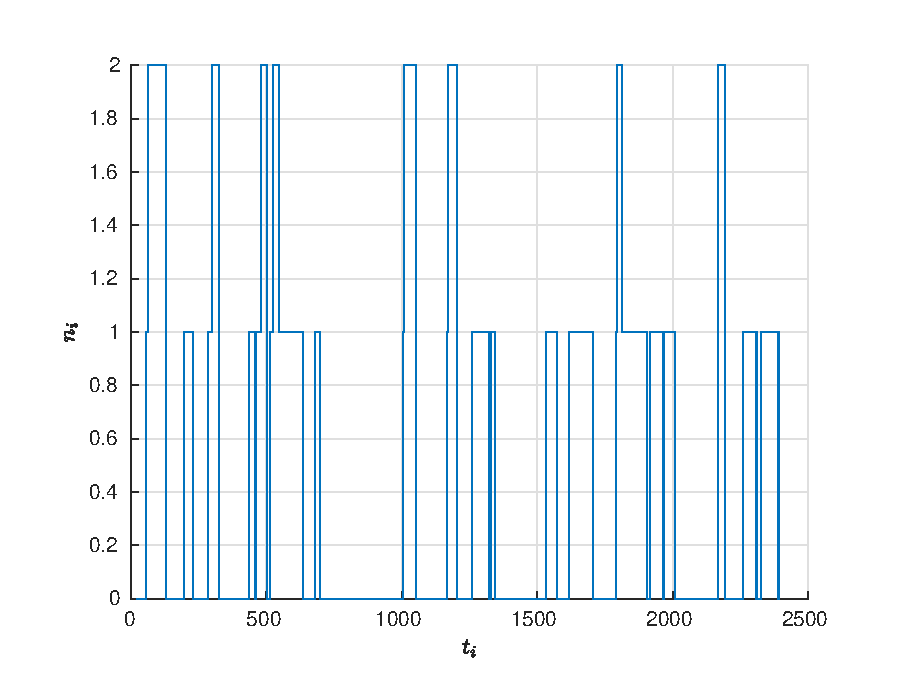
\includegraphics[width=120mm]{task_11/1-l-0-05.eps}}
        \caption{При параметре $\lambda = 0,\!05$ очередь почти не образуется.} 
\end{figure}
\begin{figure}[b]
\noindent
        \centering
        {
        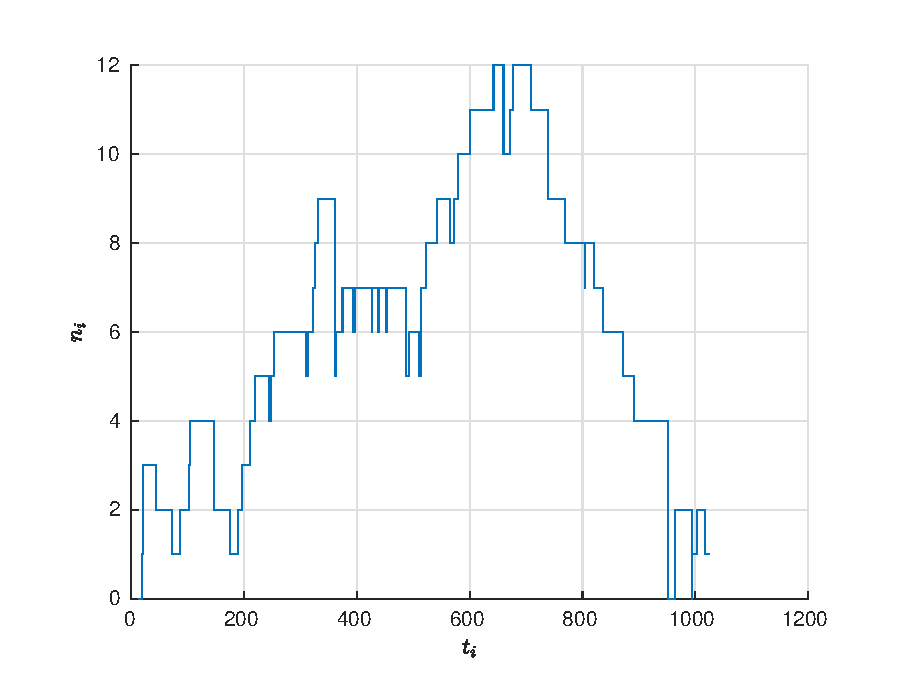
\includegraphics[width=120mm]{task_11/1-l-0-1.eps}}
        \caption{При параметре $\lambda = 0,\!1$ наблюдаем относительное равновесие. Очедь то растет, то уменьшается.}
\end{figure}
\clearpage
\begin{figure}[t]
\noindent
        \centering
        {
        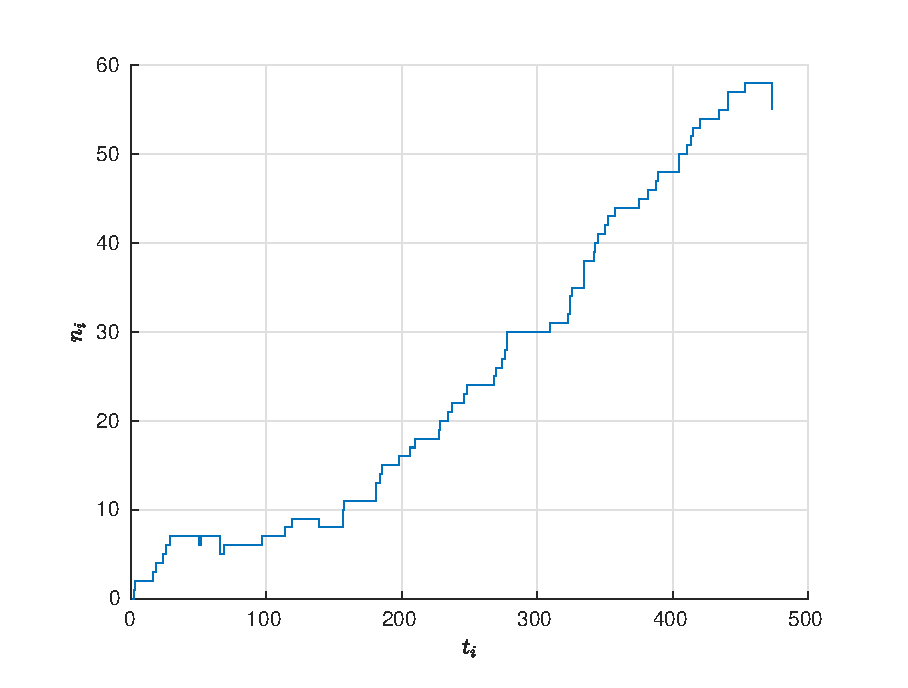
\includegraphics[width=120mm]{task_11/1-l-0-2.eps}}
        \caption{При параметре $\lambda =0,\!02$ очередь неограниченно растет.}
\end{figure}


\subsection{Система массового обслужиания с циклической интенсивностью и единичными скачками}

Пусть теперь $t_1,t_2,\ldots,t_n,\ldots$ --- времена наступления некоторых событий, $N(t_1,t_2)$ --- число событий, произошедших в промежуток времени $[t_1,t_2]$. Заметим, что $t_{i+1} - t_i$ имеет функцию распределения
$$
        F(x) = 1 - e^{-(\Lambda(t+x) - \Lambda(t))},
        \quad
        \mbox{где }
        \Lambda(t) = \int\limits_0^t\lambda(u)\,du = \lambda(t + \sin t).
$$
Здесь $x \leqslant 0$, а сам интеграл $\Lambda(t)$ неограничено возрастает при росте $t$.

Время $t_{n+1}$ распределено как $t_n + F^{-1}(U)$, где $U$ равномерно рспределенная случайная величина на отрезке $[0,1]$. Стоит отметить, что можно записать случайную величину $U$ в следующем виде:
$$
        U = 1 - e^{-E},
        \quad
        \mbox{где }
        E \sim
        \mathrm{Exp}(1). 
$$
Это соотношение позволяет сделать вывод, что $t_{n+1}$ будет распределена как $\Lambda^{-1}(E + \Lambda(t_n))$.

Мы будем искать обратную функцию к $\Lambda(t)$ численно, потому что анатически это сложно. При этом ее производная $\Lambda'(t)=\lambda_0+\lambda_0\cos(t))$ почти всюду возрастает. Такой метод моделерования неоднородного пуассоновсого процесса называется \textit{методом Льюиса-Шедлера}.

Для того,чтобы не искать обратную функцию, мы можем воспользоваться следующей модификацией этого метода. Обозначим за $t$ некоторое время --- причем нам не важно, произошло ли в это время какое-либо событие или нет. Теперь опишем алгоритм:
\begin{enumerate}
        \item Будем на каждом шаге алгоритма генерировать случайную величина $\xi$ с распределением $\mathrm{Exp}(2\lambda_0)$.
        \item Затем прибавим к переменной $t$ значение величины $\xi$ и сгенерируем новую случайную величину $\eta = \mathrm{Bern}\left(\frac{1 + \cos t}{2}\right)$.
        \item Теперь если $\eta$ приняла значение $1$, то положим $t_{i+1} = t$ и начнем слежующую итерацию ($i = i+1$). В противном случае, повторим процесс заново.
\end{enumerate}

\begin{figure}[h]
\noindent
        \centering
        {
        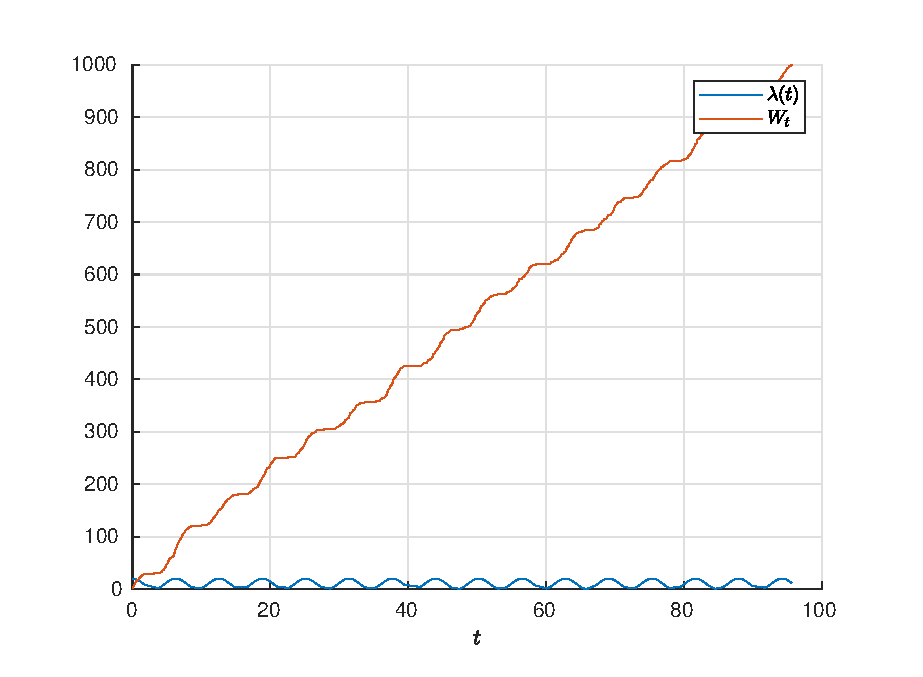
\includegraphics[width=120mm]{task_11/2.eps}}
        \caption{Cистема массового обслуживания с циклической интенсивностью $\lambda(t) = \lambda_0 (1 + \cos(t))$ и единичными скачками.}
\end{figure}


\subsection{Работа страховой компании}

\begin{definition}
        Случайная величина $\xi$ имеет \textit{распределение Парето} с параметрами $x_m$ и $k$, если ее функция распределения имеет вид
$$
        F_{\xi}(x) = 1 - \left(\frac{x_m}{x}\right)^k.
$$
\end{definition}

Для моделирования паретовской случайной величины, снова воспользуемся методом обратной функции распределения. Обратная функция имеет вид
$$
        F_{\xi}^{-1}(x)
        =
        \frac{x_m}{1-x}^{\nicefrac{1}{k}}.
$$

Будем генерировать времена наступления страховых случаев $0 \leqslant t_1 \leqslant t_2 \leqslant \ldots \leqslant t_n \leqslant T$ следующим образом:
$$
        t_i - t_{i-1} \sim \mathrm{Exp}(\lambda), \mbox{ где } \lambda > 0.
$$

Величину ущерба $s_i$ страхового случая в момент времени $t_i$ будем генерировать распределением Парето с параметрами $x_m$ и $k$. То есть по доказанному ранее будет равна $x_mU^{\nicefrac{1}{k}}$, где $U$ --- равномерно распределенная на орезке $[0,1]$случайная величина.

Величина капитала компании в момент времени $t$ выразится как
$$
        W(t) = W(0) + ct - s(t).
$$
Здесь $s(t)$ --- сумма страховых выплат до момента  времени $t$. В таком случае время разорения зададим условием:
$$
        T = \min\{t>0\;|\;W(t) < 0\}.
$$

Теперь попробуем найти зависимость между капиталом компании и параметрами $\lambda, x_m, k, W(0), c$. Если считать $k > 0$, то
$$
        \E\,W'(t)
=
        c - \E'\,s(t)
=
        c - \left(
\E\,
\sum_{t_i < t}
s_i
        \right)'
=
        c - \left(
\lambda t \E\,s_i
        \right)'
=
        c - \frac{
\lambda k x_m
        }{
k - 1
        }.
$$
В таком случае наблюдаем зависимость:
если $c(k-1) > \lambda k x_m$ --- капитал будет увеличивать, если $c(k-1) = \lambda k x_m$ --- относительное равновесие системы, $c(k-1) < \lambda k x_m$ --- капитал будет уменьшаться.
\begin{figure}[h]
        \noindent
        \centering
        {
        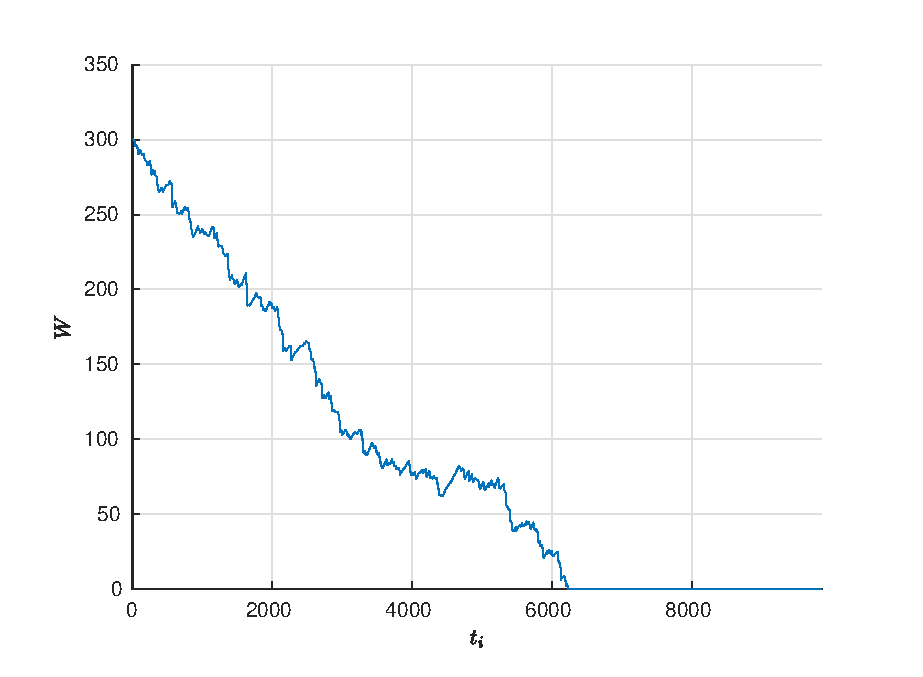
\includegraphics[width=120mm]{task_11/3down.eps}}
        \caption{Уменьшение капитала при $\lambda = 0, x_m = 1, k = 2, W(0) = 300, c = 0,\!15$.}
\end{figure}
\clearpage
\begin{figure}[t]
\noindent
        \centering
        {
        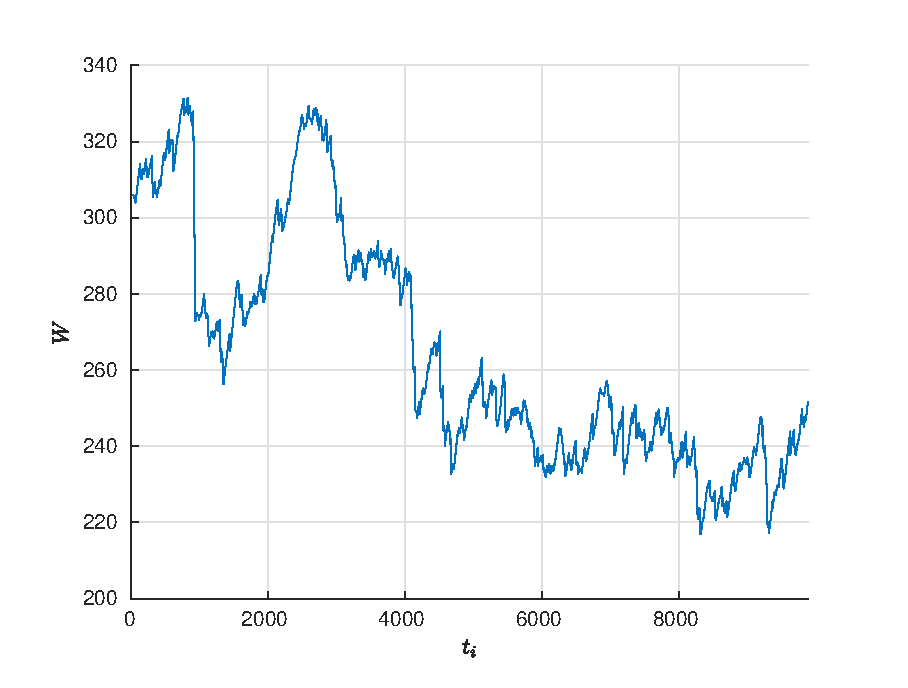
\includegraphics[width=120mm]{task_11/3equal.eps}}
        \caption{Относительное равновесие при тех же параметрах, кроме $c = 0,\!2$.}
\end{figure}
\begin{figure}[b]
\noindent
        \centering
        {
        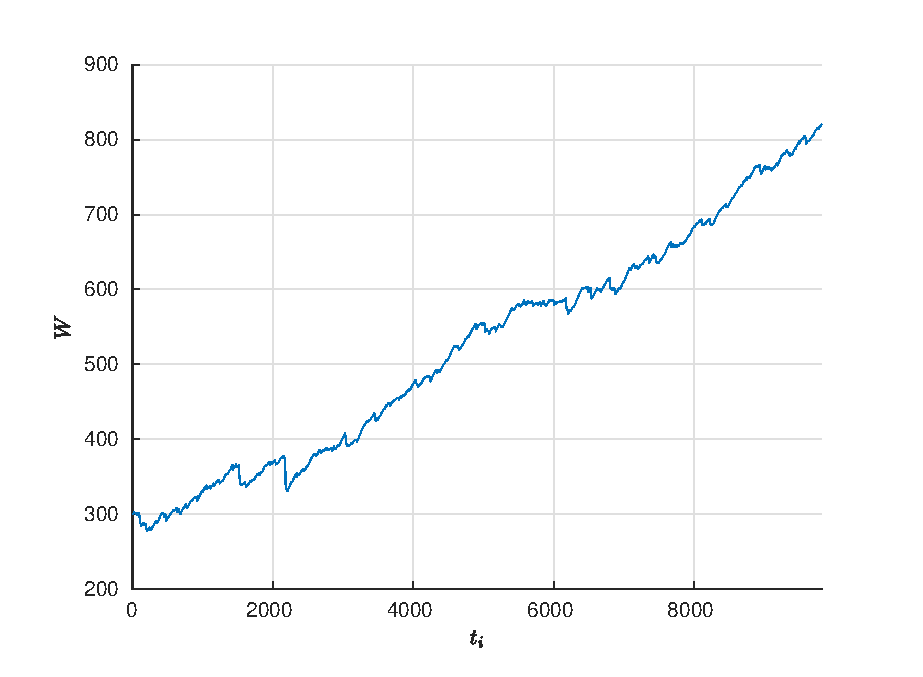
\includegraphics[width=120mm]{task_11/3up.eps}}
        \caption{Рост капитала при тех же параметрах, кроме $c = 0,\!25$.}
\end{figure}